\documentclass{article}
\usepackage{graphicx} 
\usepackage{listings}
\usepackage{geometry}


\title{Reconnaissance Faciale sur une Raspberry Pi 3 à l’aide d’une Raspberry Pi Caméra}
\author{Amir Ahmadi et Nithusan Sivakanthan}
\date{Decembre 14 2023}
\geometry{a4paper, margin=1in}
\begin{document}

\begin{titlepage}
    \centering

    \vspace{4cm}
    
    {\huge\bfseries \maketitle}

    \vspace{4cm}
    
    --------------------------------------------

    \vspace{1cm}

    Master 1 Informatique\\
    Université Paris 8\\
    Novembre 2023
\end{titlepage}

\newpage
\renewcommand{\contentsname}{Table des matières} 
\tableofcontents

\newpage


% Partie 1

\part{Introduction}

\section{Contexte}
Le projet du cours de robotique, a pour but d’implémenter  de l'Intelligence Artificielle sur un robot, ainsi nous avons décidé d'implementer sur notre robot, de la reconnaissance faciale qui peut identifié le visage de la personne si il est dans la base de données.

\section{Objectifs}% Partie 1
L'objectifs de ceux projet est de pouvoir l'utiliser dans le cadre de la sécurité, il peut etre mis en place
dans un batiment pour enregister les données d'un visage lors d'une infraction par exemple.
A notre echelle on l'utilise pour verifier si une personne detecter apartient a la liste des étudiants en M1 Informatique

\section{Definitions}
\subsection{Reconnaissance faciale}
La reconnaissance faciale est une technique qui permet à partir des traits de visage : D'authentifier une personne : c'est-à-dire, vérifier qu'une personne est bien celle qu'elle prétend être.
\subsection{Raspberry Pi}
Une "Raspberry Pi" est un nano ordinateur de la taille d'une carte de crédit que l'on peut brancher à un écran est utilisé comme un ordinateur standard
. Voici la liste des entrée et sortie de la carte:

\begin{itemize}
    \item Sortie HDMI
    \item Sortie Audio
    \item Entrées USB
    \item Entrée Micro carte SD
    \item Entrée Ethernet
    \item Entrée Module caméra
\end{itemize}

\subsection{XML}
Le XML est l'acronyme de eXtensible Markup Language, est un langage de balisage utilisé pour décrire et structurer des données de manière lisible aussi
bien par les machines que par les humains.


\part{Recherche}

\section{Environnement}

Nous avons chercher sur quelle langage développer notre projet, ainsi nous avons trouvé que le langage Python est le langagae de programmation le plus populaires
pour faire de la reconnaissance faciale. Pour ce qui est de l'editeur de texte nous avons utilisé le logiciel installé
dans l'Os Rasbian Honny-Pi.

Pour ce qui est du Materiels, nous avons decidé que une semaine sur deux, l'un de nous garder le materiels et developpé dessus, tant dis que l'autre developpe
sur ca machine personnels.
Mais au bout de quelques jours nous avons commencé a developpé sur nos machines, car les performence de la Raspberry Pi de 1Go de ram, nous ralentissez beaucoup, car
l'utilisation de la cameraPI additioné au algorithme de reconnaisance faciale prennait beaucoup de ressource, le programme prennait du temps a se lancé et parfois il arrive que la Raspberry Pi crash.
Ainsi sur nos machines,  nous developpions sur VisualStudioCode, est pour la camera, nous utilisions notre webcam.

\section{Bibliothèques}

Pour pouvoir effectuer de la reconnaissance faciale, nous avons besoin d'abord de pouvoir exploiter notre camera Pi.
Ainsi nous avons trouvé la bibliothèques "PiCamera" qui nous permet de reconnaitre et l'utilisé

Ensuite pour reconnaitre un visage nous avons trouver un fichier XML fournit pas "OpenCv" qui est aussi une bibliothèques
pour faire du traitement d'images

Nous penssions a ajouter une base de données, car pour reconnaitre une personne il faut d'abord avoir des données de cette personne
ainsi il fallait trouver un moyen d'encoder, et de stocker. Pour cela nous avons decider d'utiliser la bibliothèques "Pickle" qui va nous
permettre d'encoder des données et pour stocker les données nous avons decider d'utiliser une base de données en SqlLite



\section{Reconnaissance faciale}

\subsection{Détection du visage}

Avant de faire de la reconnaisance faciale, il faut premierement reconnaitre un visage dans une image. 
Un visage est composé de plusieurs caracteristiques tels que des yeux, sourcils, bouche, nez.

Ainsi pour ce faire la bibliothèques "OpenCV" met a disposition sur Github des fichiers XML qui contiennent des informations sur les caractiéristiques visuelles spécifiques
à un visage qui sont utilisés pour entrainer un classificateur. Ces caractéristiques sont extraites à partir d'un grand nombre d'image avec des visages et d'images sans visages.
Pour pouvoir faire de la reconnaisance de visage, nous avons donc décidé d'utilisé le fichier haarcascade-frontalface-default.xml, il va nous
permettre de reconnaitre un visage.


\begin{figure}[h]
    \centering
    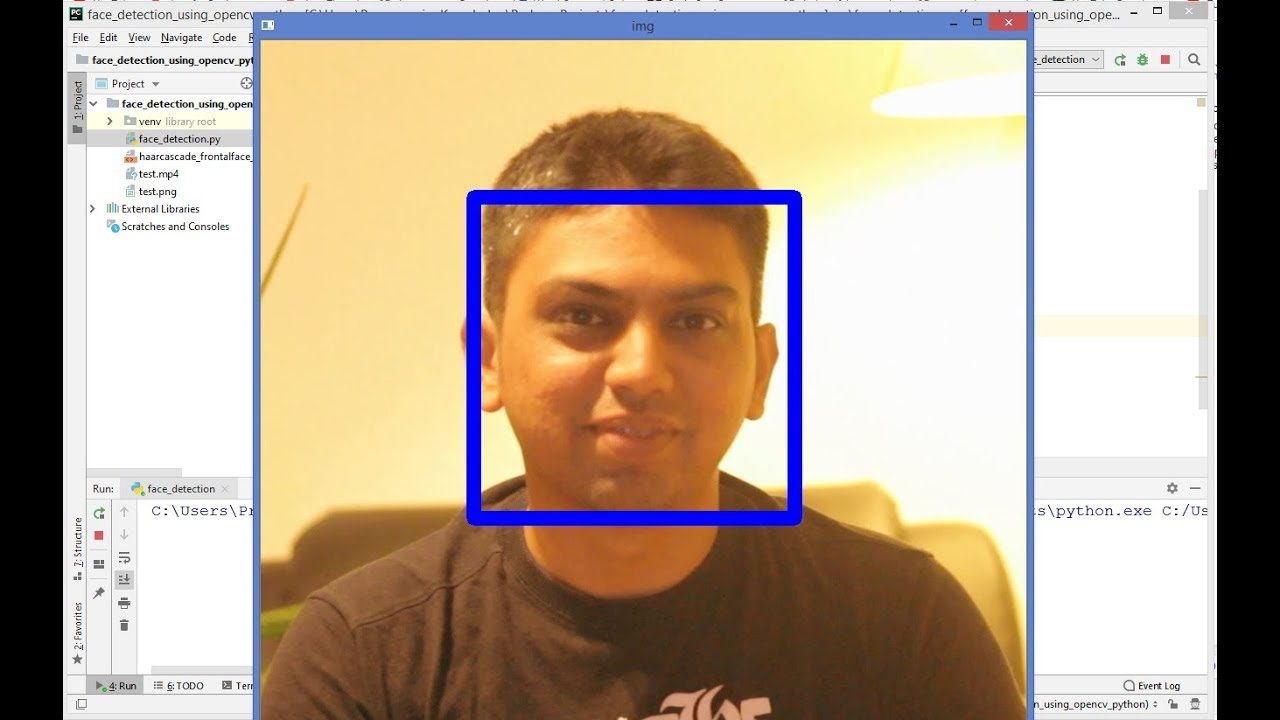
\includegraphics[width=\textwidth]{image/face_detection.jpg}
    \caption{Image montrant les différents processus de l'algorithme}
    \label{fig:mon_image}
\end{figure}

\subsection{Reconnaissance d'un individu}

Ensuite apres avoir reconnu un visage dans une image, il fallait reconnaitre a qui appartient le visage.
Pour trouver a qui correspond le visage il fallait d'abord avoir des données d'un individu sous forme d'images.

Ainsi apres avoir rassemblez plusieurs image differents du meme individu dans un seul dossier, 
il fallait entrainer un model de reconnaisance faciale avec les données de l'individu, ce qui va nous 
generer un fichier contenant les caracteristiques du visage de l'individu, c'est a dire, la position des yeux, du nez
, de la bouche ecetera.

Enfin, avec ce fichier generer, nous avons plus qu'a compare les caracteristiques du visage detecter avec  avec le fichier contenant les caracteristiques d'un individu.


\newpage
\section{Algorithme}

\subsection{Haar Cascade}

\begin{itemize}
    \item \textbf{Caractéristiques de Haar}
    \begin{itemize}
        \item L'algorithme utilise des caractéristiques de Haar,
        qui sont des filtres rectangulaires qui sont appliqués sur une région de l'image
        pour calculer la différence entre la somme des pixels dans deux zones adjacentes.
        Ces caractéristiques peuvent être des rectangles adjacents, des lignes ou des
        blocs. 
    \end{itemize}

    \item \textbf{Création d'un Classifieur}
    \begin{itemize}
        \item Un classifieur est construit en utilisant un
        ensemble d'images positives (contenant l'objet que vous souhaitez détecter, par
        exemple, des visages) et d'images négatives (ne contenant pas l'objet). Le
        classifieur est formé pour distinguer entre les deux en utilisant les
        caractéristiques de Haar. Classificateurs en Cascade : Le classifieur construit
        est ensuite organisé en une cascade de classificateurs en utilisant une
        technique d'apprentissage machine. Chaque étape de la cascade est un classifieur
        indépendant. Les classificateurs plus simples sont placés au début de la cascade,
        tandis que les classificateurs plus complexes sont placés vers la fin.
    \end{itemize}

    \item \textbf{Intégration du Classifieur}
    \begin{itemize}
        \item Une fois la cascade construite, l'algorithme
        utilise le classifieur intégré pour parcourir l'image en utilisant des fenêtres
        glissantes de différentes tailles. À chaque étape de la cascade, la fenêtre est
        évaluée avec un classifieur. Si la région échoue à une étape, elle est
        rapidement rejetée, ce qui permet d'accélérer le processus. 
    \end{itemize}

    \item \textbf{Faux Positifs et Faux Négatifs }
    \begin{itemize}
        \item Le processus peut produire des faux positifs et des faux
        négatifs. Les faux positifs sont des régions incorrectement classées comme
        positives, tandis que les faux négatifs sont des régions positives manquées. Les
        poids sont ajustés pendant le processus d'apprentissage pour minimiser ces
        erreurs. Ajustement des Classificateurs : L'algorithme ajuste automatiquement
        les seuils des classificateurs pour minimiser les faux positifs tout en
        maintenant un taux élevé de détection.
    \end{itemize}

    
\end{itemize}

\begin{figure}[h]
    \centering
    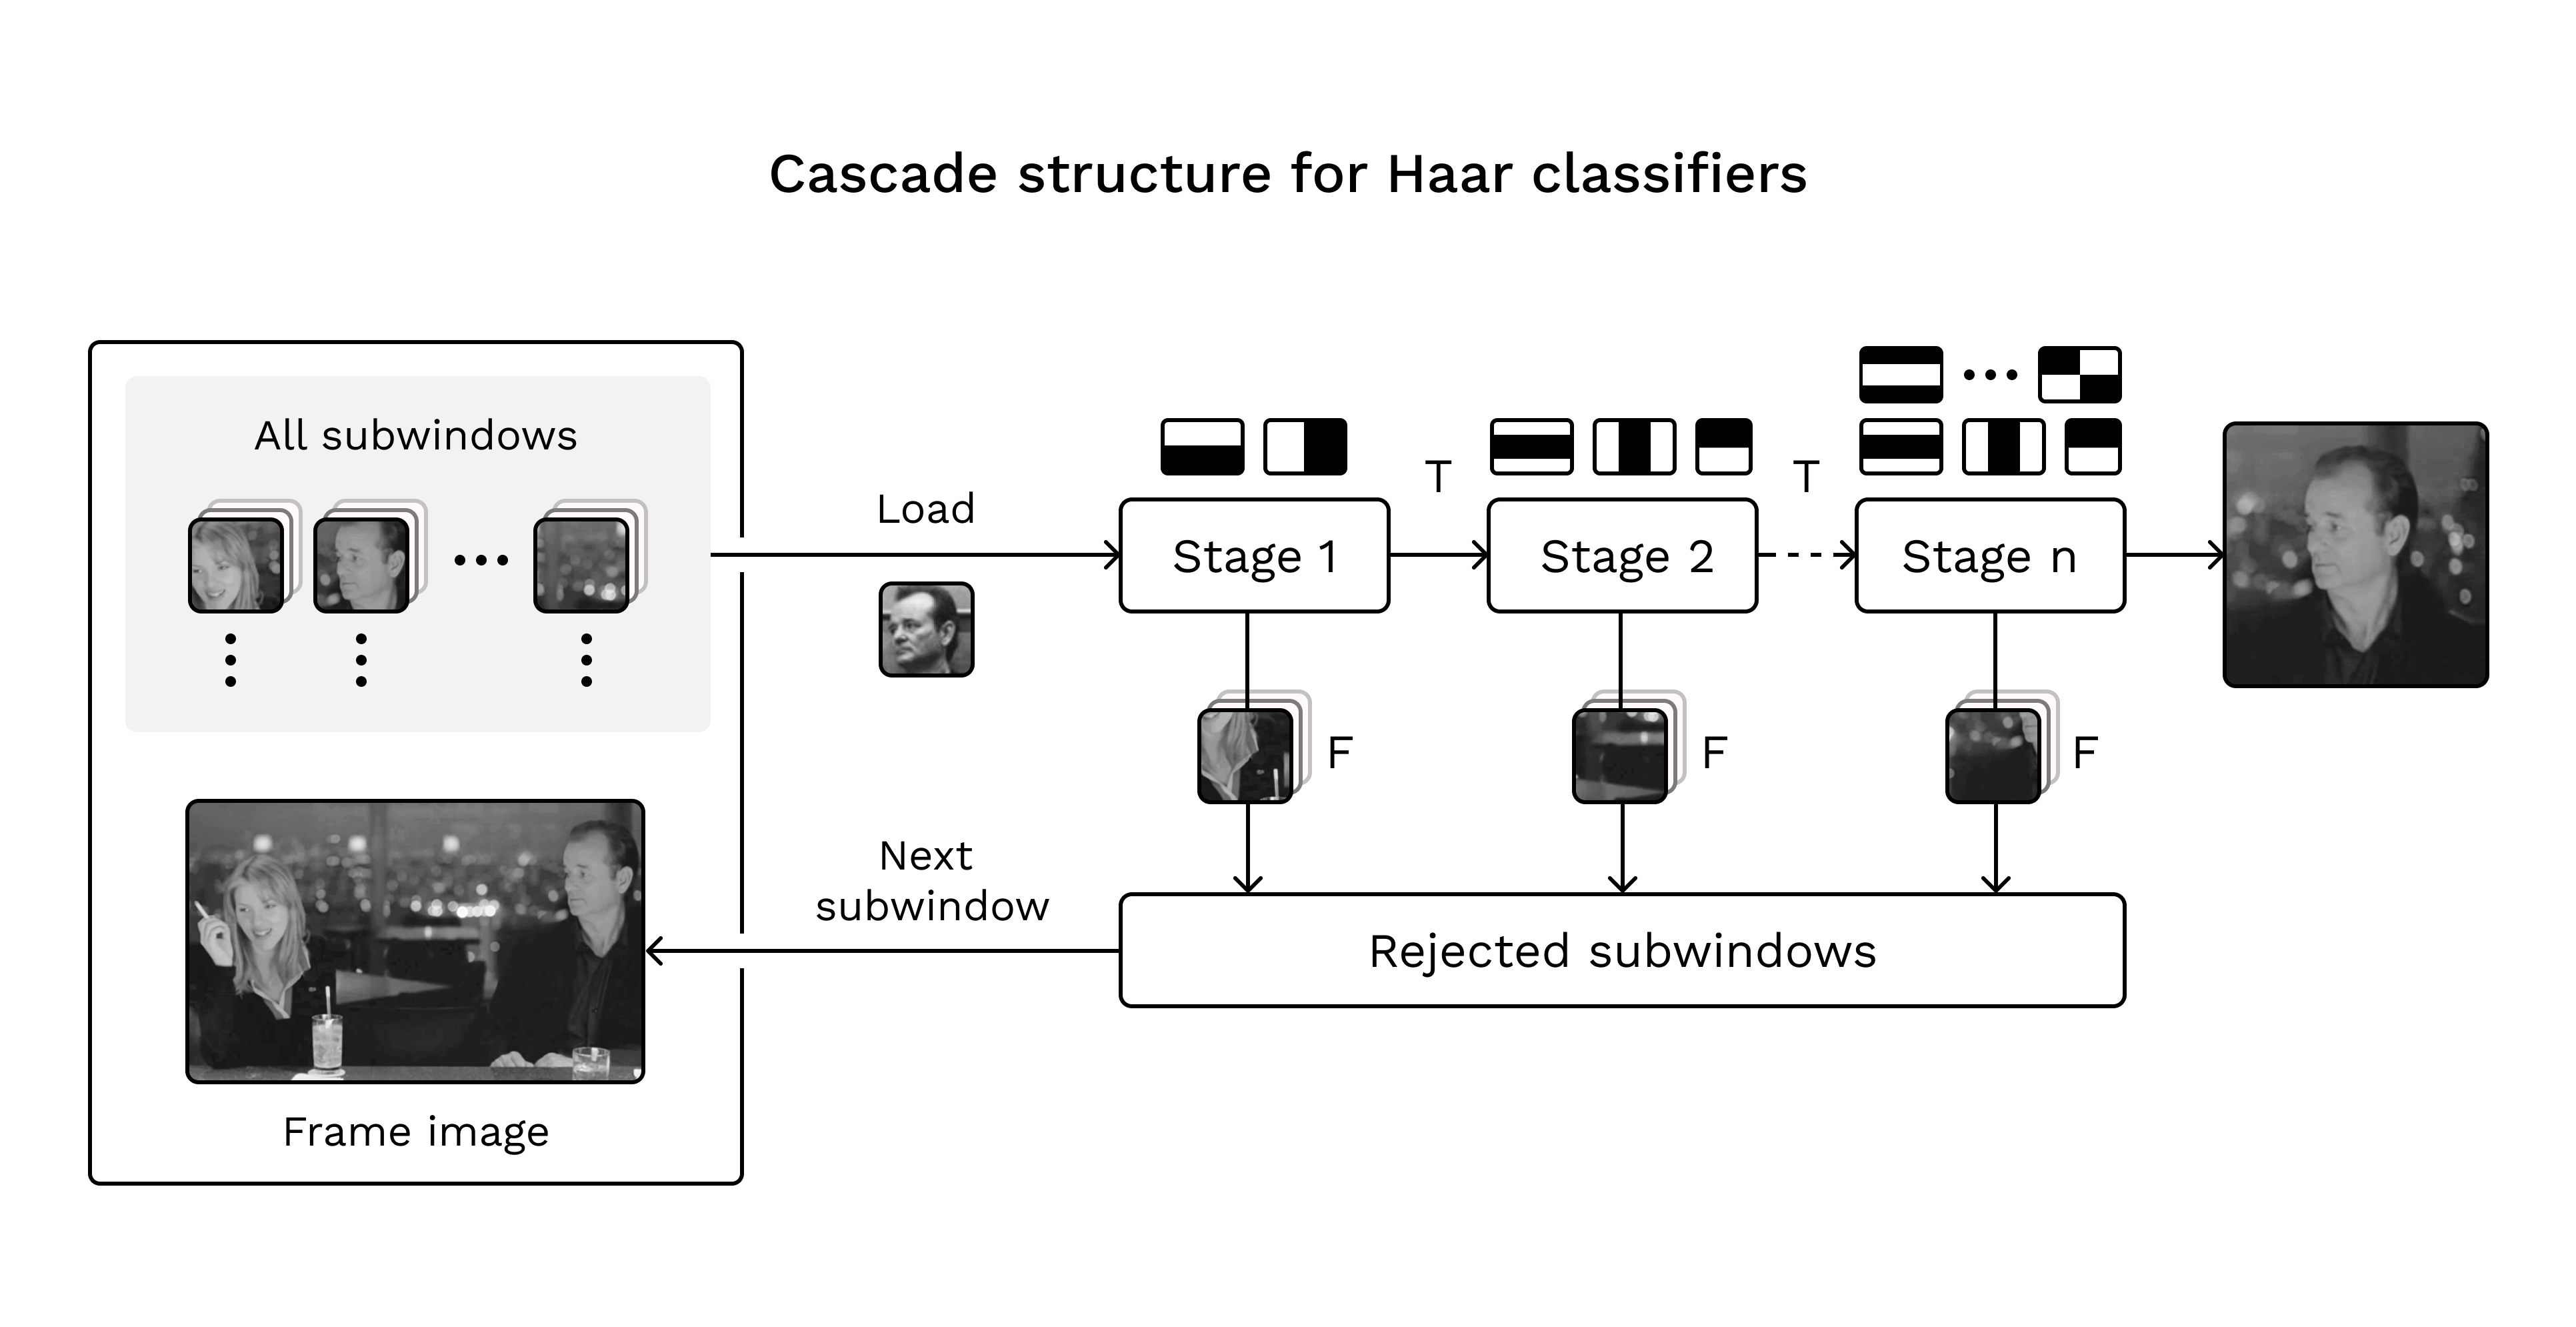
\includegraphics[width=\textwidth]{image/Cascade_structure_for_Haar_classifiers.png}
    \caption{Image montrant la détection d'un visage}
    \label{fig:mon_image}
\end{figure}
  
\part{Developpement}


\section{Materiels}
Madame Sediki nous a fournis une liste de matériels nécessaires pour réalisé notre projet, voici la liste:

% \begin{itemize}
%     \item Raspberry Pi 3
    
%     \begin{minipage}[t]{.5\textwidth} % Ajustez la largeur en fonction de vos besoins
%         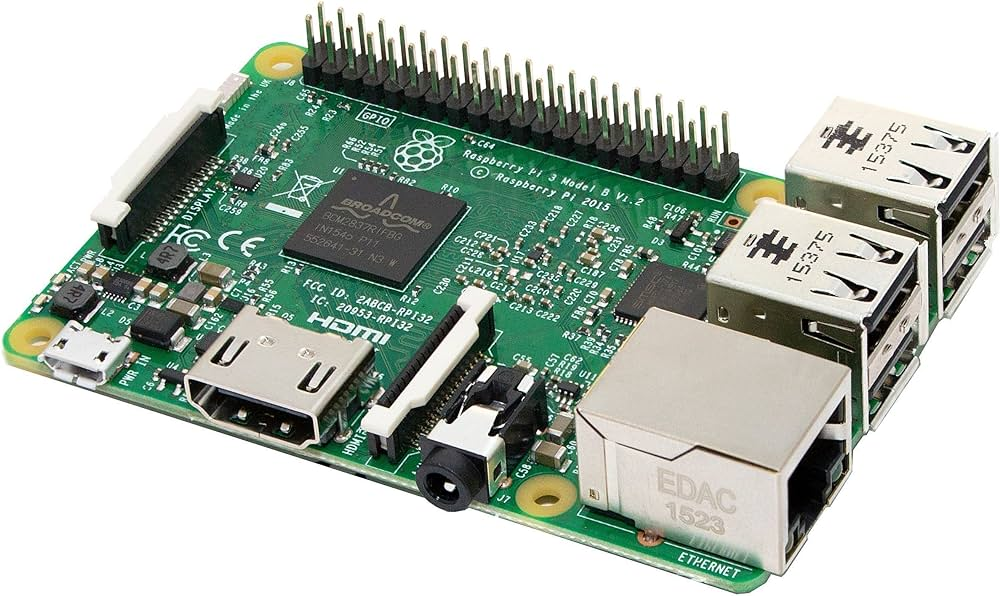
\includegraphics[width=\linewidth]{image/raspberry_pi_3.jpg} % Remplacez par le chemin de votre image
%     \end{minipage}
%     \item Adaptateur HDMI vers VGA
%     \item Carte Micro SD
%     \item Raspberry Pi Camera
%     \item Cable d'alimentation
% \end{itemize}

\begin{minipage}{0.5\textwidth}
    \begin{itemize}
    \item Raspberry Pi 3
    \item Adaptateur HDMI vers VGA
    \item Carte Micro SD
    \item Raspberry Pi Camera
    \item Cable d'alimentation
    \end{itemize}
\end{minipage}%
\begin{minipage}{0.5\textwidth}
    \vspace{20pt}
    \centering
    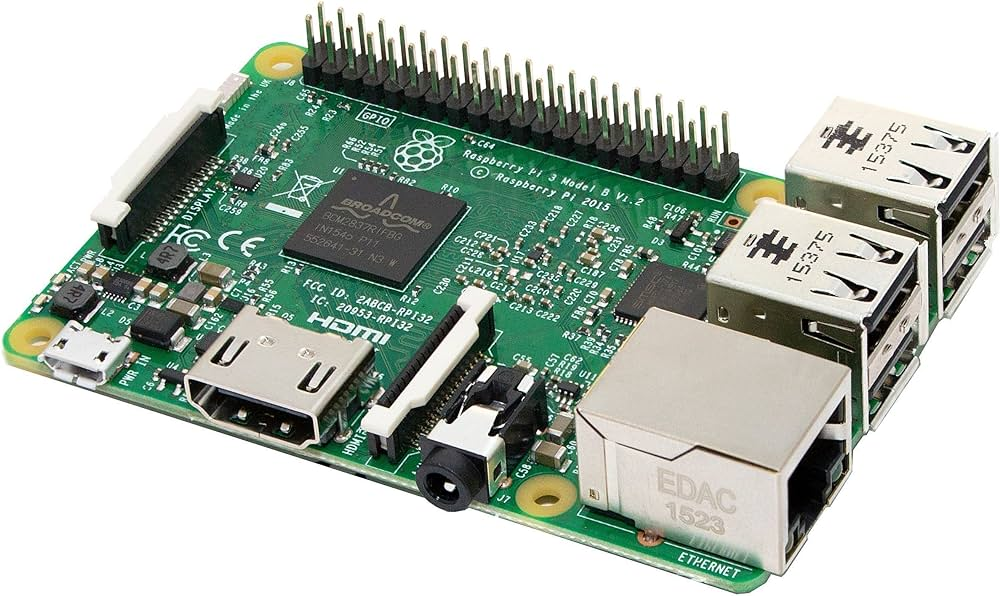
\includegraphics[width=0.8\textwidth]{image/raspberry_pi_3.jpg}
    \label{fig:tset}
\end{minipage}


\subsection{Installation}
Pour pouvoir travaillé sur la Raspberry, nous avions d'abord besoin d'installer un Os, c'est a dire un systeme d'exploitation.
Nous avions le choix entre ces deux Os :
\begin{itemize}
    \item \textbf{Raspbian}
    \begin{itemize}
        \item Raspbian est un système d’exploitation libre basé sur la distribution Linux Debian et optimisé pour le matériel de Raspberry Pi.
    \end{itemize}
    \item \textbf{Ubuntu Mate}
    \begin{itemize}
        \item Ubuntu Mate est également basé sur Debian et se révèle particulièrement utile pour avoir un ordinateur de bureau basé sur un Raspberry Pi.
    \end{itemize}
\end{itemize}
Pour notre projet, nous avons décidé d'installé Raspbian, ou plutot Raspberry Pi OS qui est son nouveau nom.
Pour se faire nous somme allé sur le site de Raspberry Pi, et avons téléchargé le version de Raspberry Pi Os Desktop, car nous avions besoin d'une interface pour pouvoir afficher le rendu de la camera.
Nous avons ensuite utiliser Etcher pour pouvoir Flashé l'Os que l'on a telechargé sur notre carte SD.
Enfin, nous inserons la carte SD dans la Raspberry Pi 3 et l'alimenton pour qu'il demarre et installe l'Os.
\subsection{Configuration}
Voici les differents commands pour finir la configuration de la Raspberry Pi.
\begin{verbatim}
    $ sudo apt-get update
    $ sudo apt-get upgrade
\end{verbatim}
\begin{itemize}
    \item \textbf{Réseau}
    \begin{itemize}
        \item Nous avions besoin du réseau, pour pouvoir faire les mise a jours du systeme et aussi pour pouvoir installer des logiciels.
    \end{itemize}
    \item \textbf{Mots de passe}
    \begin{verbatim}
        $ passwd
    \end{verbatim}
    \item \textbf{Mise à jour du système}
    \begin{itemize}
        \item Il est important de travailler sur un systeme qui est a jours pour pouvoir travailler et executer notre projet
        . Voici les commandes utilisé pour mettre a jours le systeme.
    \end{itemize}
    \begin{verbatim}
        
        $ sudo apt-get update
        $ sudo apt-get upgrade
    \end{verbatim}
    
    \item \textbf{VNC Viewer}
    \begin{itemize}
        \item Ce logiciel nous permet de controler la Raspberry Pi depuis nos machines, etant plus facile pour travailler.
    \end{itemize}
\end{itemize}

\section{Reconnaissance Faciale}

Ce bout de code va nous permettre, premierement de charger le classifieur Haar Cascade, pour nous permettre de detecter un visage 
et ensuite de dessiner un rectangle sur le visage détecter.


\newpage
\subsection{Détection du visage avec la caméra Pi}


\begin{lstlisting}[language=python, caption={Reconnaissance faciale}, label=code:exemple, numbers=left, frame=single, framerule=1pt, linewidth=\textwidth]
    
    # On recupere le classifieur
    face_cascade = cv2.CascadeClassifier(
        'haarcascade_frontalface_default.xml'
    )

    # Boucle dans lequel on affiche la camera Pi on continue
    while True:
        for frame in cam.capture_continuous(rawCapture,
                                            format="bgr",
                                            use_video_port=True):
            # On recupere la frame de la camera
            image = frame.array

            # On convertit la frame en nuance de gris
            gray = cv2.cvtColor(image, cv2.COLOR_BGR2GRAY)
            
            # Avec le classifieur on detecte les visages presents da la frame
            faces = face_cascade.detectMultiScale(gray, 1.1, 4)
            
            # On dessine un rectangle autour des visages detecter
            for (x, y, w, h) in faces:
               cv2.rectangle(image, (x, y), (x+w, y+h), (255, 0, 0), 2)
               cv2.putText(image,
                           name,
                           (x, y-10),
                           cv2.FONT_HERSHEY_SIMPLEX,
                           0.9,
                           (36,255,12),
                           2)
            # On affiche la frame avec le rectangle sur le visage
            cv2.imshow("Press", image)
            rawCapture.truncate(0)
            
            k = cv2.waitKey(30) & 0xff
            leave = False$
            if k == 27:
                print("Escape")
                leave = True
                break
            if k == 115:
                photo = photo + 1
                print(photo)
                photo_name = 'db/screen/' + name + str(photo) + ".jpg"
                print(photo_name)
                cv2.imwrite(photo_name, image)
        if leave:
            break
        
    
    cv2.destroyAllWindows()
\end{lstlisting}

\newpage
\subsection{Reconnaissance faciale}

\begin{lstlisting}[language=python, caption={Fonction chapeau va reconnaitre l'individu présent sur l'image }, label=code:exemple, numbers=left, frame=single, framerule=1pt, linewidth=\textwidth]
    def recognize_faces_video(im,
    encodings_location: Path = DEFAULT_ENCODINGS_PATH,
) -> None:
    with encodings_location.open(mode="rb") as f:
        loaded_encodings = pickle.load(f)

    face_encodings = face_recognition.face_encodings(im)

    for unknown_encoding in zip(face_encodings):
        name = _recognize_face_video(unknown_encoding, loaded_encodings)
        if not name:
            name = "Unknown"
        return name
\end{lstlisting}

\begin{lstlisting}[language=python, caption={Fonction qui va comparé les caracteristiques d'un individu avec la base de données encodé }, label=code:exemple, numbers=left, frame=single, framerule=1pt, linewidth=\textwidth]
    def _recognize_face_video(unknown_encoding, loaded_encodings):
    unknown_encoding = np.array(unknown_encoding)
    boolean_matches = face_recognition.compare_faces(
        loaded_encodings["encodings"], unknown_encoding
    )
    distance = face_recognition.face_distance(loaded_encodings["encodings"],
                                              unknown_encoding)
    
    list_distance = list(map(lambda x: round(x * 100), distance))
    list_accuracy = list(map((lambda x: 100 - x), list_distance))
    list_validation = list(
        map((lambda ac: True if ac >= 50 else False),list_accuracy))
    
    votes = Counter(
        name
        for match, name in zip(list_validation, loaded_encodings["names"])
        if match
    )
    if votes:
        return votes.most_common(1)[0][0]
\end{lstlisting}

On peut voir ligne 10 que l'on calcule la distance, il s'agit de la du pourcentage de ressemblence entre chaques caracteristiques des individus present l'encodage et l'individu present
dans la frame de la webcam, ensuite ligne 11 je construit une liste qui remplit met false si la ressemblence est inferieur a 50 sinon true a l'index correspondendant aux données de l'individue.

Exemple: [ true, false, true , false, false] equivalent à [ Nithusan, Amir, Nithusan, Amir, Amir].

Ainsi, ligne 14 je compte le nombre de fois ou true apparait pour chaque individu, dans mon exemple cela va me donné
votes = { Nithusan: 2, Amir: 0}.

Enfin je retourne l'individu qui a le plus de caracteristiques en commun de ma liste encodé.

    

\newpage
\section{Base de données}

Il nous faut maintenant une base de données sur lequel l'algorithme Haar Cascade compare ces données de visage avec ceux 
des individues qu'on a creer, pour un base de données en SqlLite.

... Parti Amir Explication ...





\subsection{Encodage des données des individus}

Avant avoir creer une base de données d'individu, il nous fallait maintenant pouvoir transcrire les données des visages pressent sur chaque images dans un fichier.
Ainsi nous avons creer une fonction qui parcourt une liste d'image donné, pour chaque 
image, on utilise la biblioteque face-recogntion pour localiser sur l'image le visage de l'individu et encoder les caracteristiques du visage de l'individu dans
un fichier Pickle. 

\begin{lstlisting}[language=python, caption={Fonction qui encode les caracteristiques du visage d'un indivudu}, label=code:exemple, numbers=left, frame=single, framerule=1pt, linewidth=\textwidth]
    
    def encode_images_faces(name, images,
    model: str = "hog") -> None:
    
    encodings = []
    names = []
    name = name.split(" ")
    name = name[0] + "_" + name[1]
    encodings_location: str = Path(f"db/encoding/liste_personne/{name}.plk") 
    for image_file in images:
        face_reco_image = face_recognition.load_image_file(image_file)

        face_locations = face_recognition.face_locations(face_reco_image,
                                                         model=model)
        face_encodings = face_recognition.face_encodings(face_reco_image,
                                                         face_locations)

        for encoding in face_encodings:
            names.append(name)
            encodings.append(encodings)
        
    names_encodings = {"names": names, "encodings": encodings}

    with encodings_location.open(mode="wb") as f:
        pickle.dump(names_encodings, f)
    
    return encodings_location
\end{lstlisting}


% Partie 3
\part{Résultats}
\section{Analyse des résultats}


% Partie 3

\part{Conclusion}

Pour conclure, nous avons reussi a faire de la reconnaissance faciale a l'aide de la camera Pi, ce projet nous a donné un avant de gouts
du fonctionnement de la reconnaissance faciale.

\end{document}